\documentclass[letterpaper,12pt]{article}
\usepackage[utf8]{inputenc}
\usepackage[bottom]{footmisc}
\usepackage{graphicx}
\usepackage{amsmath}
\usepackage{amsthm}
\usepackage{amscd}
\usepackage{amssymb}
\usepackage{latexsym}
\usepackage{upref}
\usepackage[hidelinks]{hyperref}
\usepackage{cite}
\usepackage{subcaption}

\setlength{\textwidth}{6.4in}
\setlength{\textheight}{9.5in}
\setlength{\topmargin}{-1in}
\addtolength{\headheight}{0.0675in}
\setlength{\oddsidemargin}{0.2in}
\setlength{\evensidemargin}{0.2in}

\begin{document}

    \title{
        A Deep Learning Approach to Solving Hyperbolic PDEs\\
    }
    \author{%
        Thompson, J.
    }
    \date{\today}
    \maketitle

    \begin{abstract}
        In this project, we examine a deep learning approach to solving various hyperbolic equations, including 
        (but not limited to) a basic advection equation and the one-dimensional inviscid Burgers equation.
        Such equations arise naturally in the study of fluid and traffic flows and are solvable via traditional 
        finite difference approaches. Numerical solutions are therefore readily available (or may be easily generated),
        and so the problem of data collection for deep learning is well-mitigated.
    \end{abstract}


    \section{Background}\label{sec:background}
    Recent advancements in the field of machine learning have led to the development of Physics-Informed Neural 
    Networks (PINNs), wherein a neural network is used as a solution surrogate to systems of partial differential 
    equations (PDEs). Such networks are typically trained from available sparse data; typically, the amount of data
    available to train a neural network is insufficient for a neural network to converge. However, by encoding the 
    governing PDE term into the network training process (either by including the PDE residual into network training as
    in a multi-objective approach or by some other scheme), recent empirical successes indicate that
    sparse data and/or specified boundary conditions provide sufficient convergence conditions for the neural network to
    successfully approximate the true PDE solution.\cite{raissi_physics-informed_2019} In fact, neural networks are 
    particularly well-suited to solve the inverse problem for PDEs - that is, to infer some unknown parameter of 
    function which is part of the original system of PDEs.\cite{lu_deepxde_2021} In this project, we propose to utilize
    PINNs to solve both the forward and inverse problem for two well-known hyperbolic PDEs. The first of these is a 
    standard advection equation, which is perhaps the simplest possible hyperbolic PDE:

    $$
    u_t + a u_x = 0
    $$

    \ \\
    \noindent for some constant $a$ and initial condition $u(x, 0) = u_0(x)$. The second equation we will examine is the
    inviscid Burgers' equation, which we obtain by letting $a = u$ from above:

    $$
    u_t + u u_x = 0
    $$

    \section{Methodology}\label{sec:proposed-methodology}

    In this project, we utilize DeepXDE\footnote{
        Source code for this library may be found at
        \hyperlink{https://github.com/lululxvi/deepxde}{https://github.com/lululxvi/deepxde}
    }, a Python framework built on top of Tensorflow for scientific machine learning and physics-informed 
    learning.\cite{lu_deepxde_2021} DeepXDE solves PDEs by embedding the PDE residual term into the loss term of the
    neural network solution approximation. For the forward solution (i.e., with specified initial and boundary 
    conditions), the resulting neural network takes spatiotemporal data as input and outputs the predicted solution 
    value at each point. PINNs typically operate well with 1-3 hidden layers, though one aim of this project is to 
    determine which neural network architecture(s) lead to convergent system solutions. For the inverse problem, we will
    generate training data for both advection and inviscid Burgers' equations via known solutions for particular values
    of $a$ and initial condition $u_0(x)$ to determine these values from sampled solution data. In general, we 
    define a general non-linear partial differential equation as follows:

    $$
    u_t + N[u; \lambda] = 0, x \in \Omega, t \in [0, T]
    $$

    \ \\
    \noindent where $u(x, t)$ solves the PDE, $N[\cdot, \lambda]$ denotes some non-linear differential operator, and 
    $\lambda$ may represent some unknown (learnable) parameter(s) in the non-linear PDE. To determine a numerical PINN 
    solution to the PDE, we substitute a neural network $\mathcal{NN}(x, t; \lambda)$ solution surrogate for $u(x, t)$. 
    We do so by utilizing \textit{multi-task learning}, wherein we optimize for two distinct objectives. The first of 
    these objectives - unique to PINNs - is to minimize the PDE residual:

    $$
    L_{res} = ||u_t + N[u; \lambda]||
    $$

    \ \\
    For the PDEs discussed at present, we will find that this loss term (when encoded with appropriate boundary 
    conditions) is often sufficient to solve the PDE in the forward case. When observed measurement data for the PDE 
    is available (perhaps by way of some physical sensor array), we may utilize an additional, more conventional loss 
    term which penalizes the neural network solution for failing to satisfy observed measurements:

    $$
    L_{obs} = ||u - \hat{u}||_{\Gamma}
    $$

    \ \\
    \noindent where $\hat{u}$ represents (generally sparse) measured data at various points 
    $\Gamma \in \partial \Omega \cup \Omega$ in the domain. In general, then, our problem reduces to finding appropriate
    neural network parameters $\lambda$ which minimize this aggregate loss:
    
    $$
    \min_{\lambda}{||L_{obs} + L_{res}||}
    $$

    We do so first by way of the Adam\cite{adam} algorithm to find candidates for global minima and then L-BFGS to 
    narrow in on our solution candidate. Lastly, we utilize the hyperbolic tangent activation function in our neural 
    network in order to satisfy smoothness requirements for PDEs.

    % \section{Goals and Objectives}\label{sec:goals}
    % We hope to utilize neural networks to solve an advection and inviscid Burgers equation with a known reference 
    % solution. Moreover, we hope to analyze the applicability of the learned equation to similar systems in order to 
    % determine whether the trained neural network provides robustness and/or generalizability beyond that of the provided
    % training data set. For the inverse problem in the advection equation, we will examine the trained network's ability 
    % to predict values of $a$ from other initial conditions. Furthermore, if time allows, we will examine the utility
    % of PINNs in solving the viscid Burgers' equation in both forward and inverse cases with residual-based
    % adaptive refinement to account for the sharp front:

    % $$
    % u_t + u u_x = \nu u_{xx}
    % $$

    \section{Advection Equation}{\label{sec:advection-equation}}
    We begin with the 1D advection equation. This equation serves as a useful model for describing the movement of some
    material by way of ambient fluid velocity. If we suppose that our system takes place in a one-dimensional donut and
    wrap our domain in a circle (with the assumption that advected material moves in a single direction), we ought to
    expect that such a system gives rise to a periodic boundary condition, i.e., $u(0, t) = u(1, t)$. Our problem
    statement then becomes:

    $$
    u_t + a u_x = 0, \Omega = [0, 1] \times [0, 1], u(0, t) = u(1, t), u(x, 0) = \eta(x)
    $$


    \ \\
    Solutions to this equation are given by:

    \begin{align*}
    u(x, t) = \begin{cases}
        \eta(x - at), &a > 0, \\
        \eta(x + at), &a < 0, \\
        \eta(x), &a = 0,
    \end{cases}
    \end{align*}


    \subsection*{Forward Solution}{\label{sec:advection-equation-forwared}}
    To solve this equation via a PINN, we utilize a neural network with three hidden layers and 12 neurons in each 
    layer. Because we are solving this equation forward in time, we do not have any pre-existing measurement data from
    which to train. As such, our optimization target reduces solely to the PDE residual and corresponding boundary
    conditions.


    \begin{figure}[h]
        \centering
        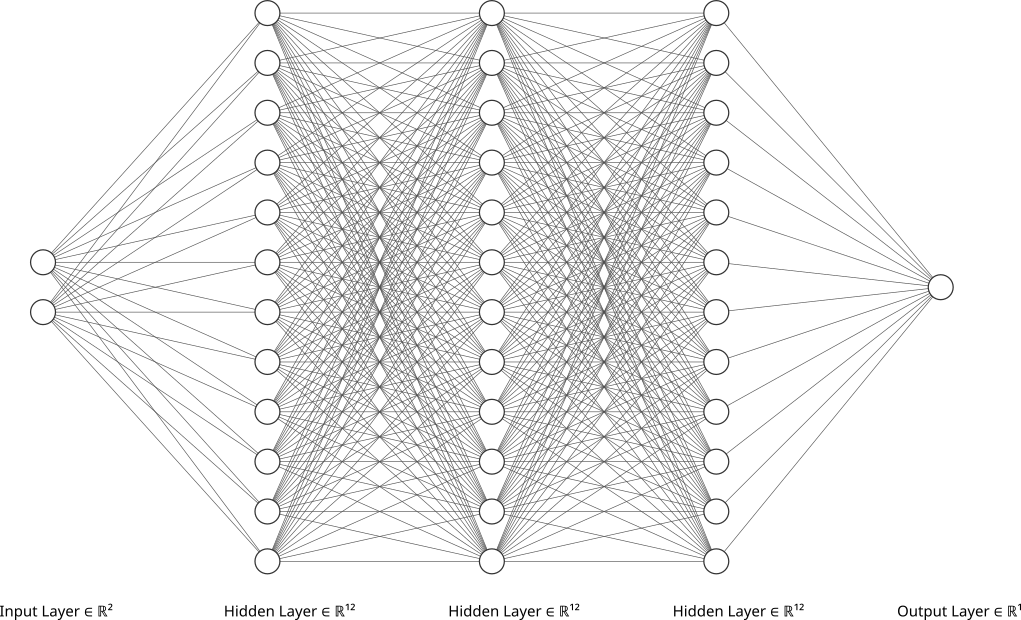
\includegraphics[width=0.70\textwidth]{nn.png}
        \caption{Advection equation network architecture with inputs $x, t$ and output $u$}
    \end{figure}

    We train our solution on a grid with 400 and 20 randomly distributed spatial and temporal points respectively and
    impose a Gaussian initial condition:
    $$
    \eta(x) = e^{-(4x)^2}
    $$
    
    We find that the neural network solution converges after 10000 iterations with a mean residual on the order of 
    $10^{-4}$ and L2 relative error on the order of $10^{-2}$. Of particular interest is the fact that the neural 
    network solution performs quite well outside the original temporal domain; in fact, we observe that while the neural
    network is trained to optimize the PDE residual on $t \in [0, 1]$, the learned solution closely mathces the exact 
    solution up until $t=3$. This suggests that the neural network learns (to some degree) that solutions to the 
    advection equation consist of traveling wave packets.

    \begin{figure}[h]
        \centering
        \begin{subfigure}{0.45\textwidth}
            \includegraphics*[width=\textwidth]{advection_forward_t0.00.png}
            \caption{$t = 0$}
        \end{subfigure}
        \hfill
        \begin{subfigure}{0.45\textwidth}
            \includegraphics*[width=\textwidth]{advection_forward_t1.00.png}
            \caption{$t = 1$}
        \end{subfigure}
        \begin{subfigure}{0.45\textwidth}
            \includegraphics*[width=\textwidth]{advection_forward_t2.00.png}
            \caption{$t = 2$}
        \end{subfigure}
        \hfill
        \begin{subfigure}{0.45\textwidth}
            \includegraphics*[width=\textwidth]{advection_forward_t3.00.png}
            \caption{$t = 3$}
        \end{subfigure}
    \end{figure}

    \subsubsection*{Comparison with Finite Differences}
    Advection equations are notoriously difficult to solve by standard numerical schemes due to the presence of
    discontinuous shock solutions. In particular, finite difference methods for the advection equation typically require
    careful discretization in order to prevent the introduction of numerical oscillations, damping, or instability.
    
    PINNs, as we shall see, handle this quite well. For the present purposes, it is of interest to note that the 
    formulation of PINNs as a constrained optimization problem allows for arbitrary meshes from which to sample training
    points \footnote{
        There is most assuredly some lower limit to this, though that limit naturally depends on the problem and domain 
        under consideration.
    }. As such, PINNs fall into the class of \textit{meshfree} numerical methods. In particular, this eliminates
    the need to correlate spatial and temporal discretizations in a particular way, e.g., by enforcing compliance with
    the Courant-Friedrichs-Lewy (CFL) condition. We demonstrate this explicitly by intentionally introducing an unstable
    finite difference grid by sampling $n^2$ spatial points - where $n$ is the number of temporal points - in the 
    forward advection solution.

    \subsection*{Inverse Solution}
    It should be noted that the introduction of multiple training targets can sometimes introduce competing gradient 
    optimizations - in other words, satisfying $L_{obs}$ more closely sometimes incurs increased loss from the $L_{res}$
    term or vice versa.

    \pagebreak
    \nocite{*}
    \bibliographystyle{plain}
    \bibliography{refs}


\end{document}
